% !TeX root = main.tex
\section{Inertial frames, principles of relativity, the Galilean transformation, the Lorentz transformation and its consequences}
\label{sec:inertial-frames}

    An inertial frame is a frame of reference with respect to which every body, not subject to external interactions with other bodies, moves in uniform rectilinear motion or remains at rest. The existence of such a frame is postulated by Newton's first law of motion.

    The Galilean principle of relativity states that the laws of motion are identical in all inertial frames of reference, i.e.\ there is no privileged frame of reference. It was formulated in 1604 in the form of the following law: all frames of reference moving with respect to one another at constant velocity (including $\vec{v}=0$) are equivalent. Its consequence is the set of Galilean transformations between two frames of reference $(t,x,y,z)$ and $(t',x',y',z')$ with the primed one moving with velocity $v$ with respect to the unprimed one along the $x$ axis:

    \begin{equation}\label{eq:gallilean}
        \begin{aligned}
            t' &= t \\
            x' &= x - vt \\
            y' &= y \\
            z' &= z
        \end{aligned}
    \end{equation}

    Einstein additionally postulated that in every inertial frame of reference the speed of light must have the same value. He made this assumption in 1905 based on an analysis of the transformations of Maxwell's equations, where he found that magnetic and electric field may be interchanged on the transofrmation of coordinate system.
    \todo{Language}

    The Galilean transformations were thereby generalised to the Lorentz transformation to accommodate the Einstein's postulate:

    \begin{empheq}[box=\fbox]{equation}\label{eq:lorentz}
        \begin{aligned}
            t' &= \gamma\left(t-xv/c^2\right) \\
            x' &= \gamma\left(x-tv\right) \\
            y' &= y \\
            z' &= z
        \end{aligned}
    \end{empheq}

    where the parameter $\gamma$ is known as the Lorentz factor:

    \begin{equation}\label{eq:gamma}
        \gamma = \frac{1}{\sqrt{1 - \beta^2}} > 1,\quad \beta=\frac{v}{c},
    \end{equation}
    
    Note that in the limit $\nicefrac{v}{c} \xrightarrow{} 0$ the transformation reduces to the Galilean transformation (\cref{eq:gallilean}).

    \needspace{4\baselineskip}
    The consequences of the Lorentz transformation include:
    \begin{enumerate}
        \item Time dilation, described by the formula $\Delta t = \gamma\Delta t_0$, where $\Delta t_0$ is the \emph{proper time}---time recorded in the rest frame of the timed event, and $\Delta t$ is the time recorded by another observer moving with velocity $v$ with respect to the first. \emph{The event appears \emph{shortest} in its own frame.}
        \item Lorentz contraction, described by the formula $L = {L_0}/{\gamma}$, where $L_0$ is the \emph{proper length}---length of an object at rest, and $L$ is the length of the object recorded by an observer moving with respect to it at velocity $v$. \emph{The object appears \emph{longest} in its own frame.}
        \item Relativity of simultaneity: two events determined by one observer to be simultaneous need not be simultaneous for another observer. Simultaneity translates to other frames only for the events that happen at the same point in space.
        \item The description of vector quantities in four dimensions. Position, momentum and potential are described respectively by a four-vector, a four-momentum and a four-potential. For example:
        \todo{elaborate a little}
        \begin{equation*}
            p^{\mu} =
            \begin{bmatrix}
                p^{0} \\ p^{1} \\ p^{2} \\ p^{3}
            \end{bmatrix}
            =
            \begin{bmatrix}
                E/c \\ p_x \\ p_y \\ p_z
            \end{bmatrix}
        \end{equation*}
    \end{enumerate}

\section{Fundamental interactions; carriers and range of interactions, charges and characteristic energy scales}

    Four types of fundamental interaction are currently known, each mediated by its own carrier:

    \begin{itemize}
        \item the strong interaction
        \item the weak interaction
        \item the electromagnetic interaction
        \item the gravitational interaction
    \end{itemize}

    In quantum theories, interactions are transmitted by certain particles called interaction carriers or interaction quanta. There are two categories of such particles---real particles (transmitting the fundamental interactions) and quasiparticles (pseudoparticles: the phonon, the plasmon, the magnon).

    \begin{table}[h!]
        \centering
        \begin{tabular}{|c|c|c|c|c|c|}
            \hline
            interaction & carrier & range & charge & mass & spin \\
            \hline
            strong & gluon & $10^{-15}$\,m & colour & 0 & 1 \\
            \hline
            weak & $W^+, W^-, Z^0$ boson & $10^{-18}$\,m & isospin & $m_0>0$ & 1 \\
            \hline
            electromagnetic & photon & $\infty$ & --- & 0 & 1 \\
            \hline
            gravitational & graviton (hypothetical) & $\infty$ & --- & 0 & 2 \\
            \hline
        \end{tabular}
    \end{table}\todo{bolder line at the top; add hydrogen atom size for reference}

    Energies here are quoted in \emph{electronvolts}: $1$~eV is the energy an electron gains on being accelerated through a potential difference of one volt, $1\,\mathrm{eV} = 1.602\times10^{-19}$~J, with the usual multiples keV, MeV and GeV. Masses are quoted in the same units, which is possible because of \emph{mass--energy equivalence}, $E = mc^{2}$: a mass is given by the rest energy it corresponds to. Strictly this makes the unit of mass the eV$/c^{2}$, but the $c^{2}$ is almost always left out and one simply says that the $W$ boson has a mass of $80$~GeV. In SI units $1$~eV$/c^{2} = 1.783\times10^{-36}$~kg.

    The ranges in the table are not independent facts: they follow from the masses of the carriers, by the following order-of-magnitude argument. The energy--time uncertainty relation, $\Delta E\,\Delta t \geq \hbar/2$, says that a state which exists only for a short time cannot have a sharply defined energy. Note what it is about: the spread of energy of a short-lived state itself, not the precision of our measurements, and not the mass of the particle species, which is a fixed number obtained from real particles produced in accelerators.

    A carrier exchanged between two particles is never observed directly, and so is not obliged to balance the energy books: it may in effect be borrowed from the vacuum, provided the loan is repaid quickly enough. Borrowing at least the rest energy $mc^{2}$ of the carrier limits its life to $\Delta t \sim \hbar/mc^{2}$, and moving at most at the speed of light it can cover a distance

    \begin{equation}\label{eq:yukawa-range}
        R \sim c\,\Delta t \sim \frac{\hbar}{mc},
    \end{equation}

    the Compton wavelength of the carrier. A heavy carrier therefore gives a short-ranged force and a massless one an unlimited range, which is why electromagnetism and gravitation reach as far as they do. For the weak interaction, $\hbar c \approx 197$~MeV~fm divided by a carrier rest energy of about $80$~GeV gives $R \approx 2\times10^{-18}$~m, the figure in the table.

    The strong interaction is the exception, since its carrier is massless and yet the force does not reach beyond the nucleus. Its range is set instead by \emph{confinement}: colour charge cannot be isolated, so gluons never travel freely between well-separated particles. What acts between nucleons is a residual force carried by pions, of rest energy about $140$~MeV, and the same estimate then gives the familiar $1.4\times10^{-15}$~m.

    \begin{figure}[h]
        \centering
        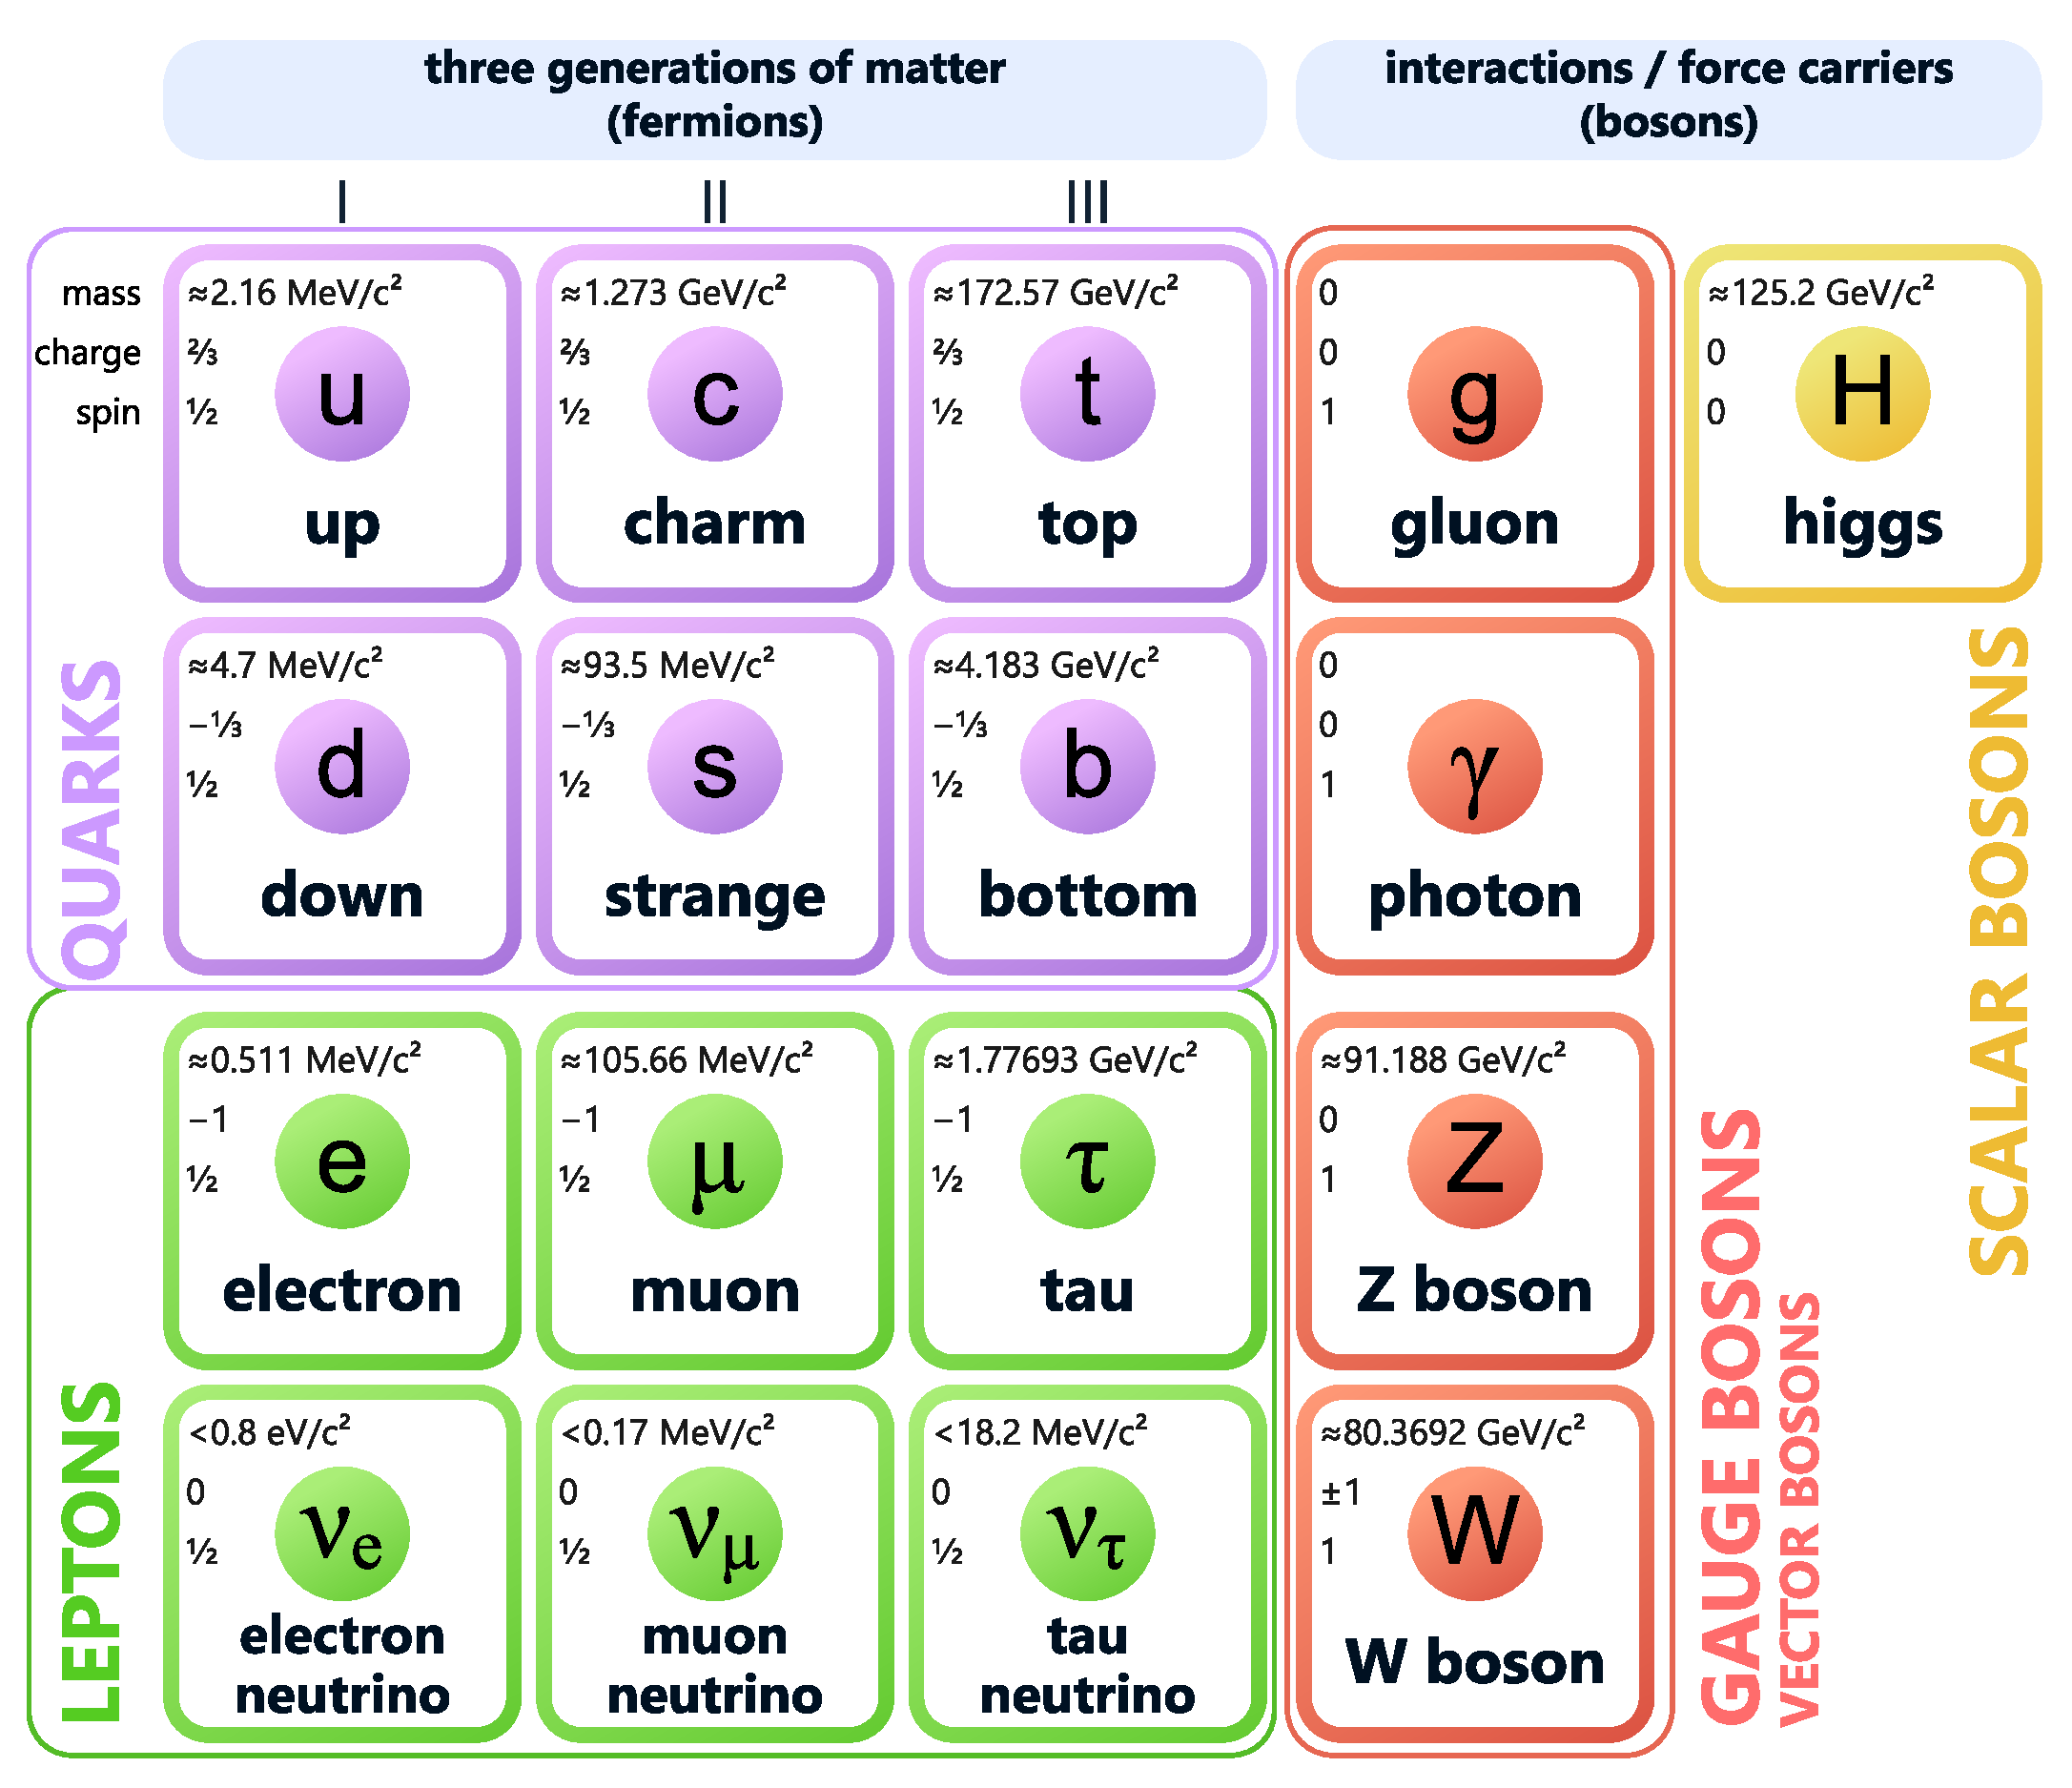
\includegraphics[width=0.6\linewidth]{graphics/Standard_Model_of_Elementary_Particles.pdf}
        \caption{Standard Model of Elementary Particles.}
        \label{fig:standard-model-particles}
    \end{figure}

    Intermediate bosons are exchanged by electrons, neutrinos and other particles participating in the weak interaction during collisions. The $W$ boson occurs in two basic forms: the particle $W^+$ and its antiparticle $W^-$. Both have the same spin and mass, $80.369 \pm 0.013$~GeV, and differ only in electric charge. The $W$ bosons carry one of the charges of the electroweak interaction, namely weak isospin. Its value is $+1$ and $-1$ for the $W^+$ and $W^-$ bosons respectively. The most important phenomenon involving $W$ bosons is beta decay. In this process a down quark (d) contained in a neutron decays into an up quark (u) and a $W$ boson, which in turn decays into a lepton--neutrino pair for a given lepton (more precisely: $W^-$ decays into a lepton plus an antineutrino, and $W^+$ into an antilepton plus a neutrino). As the energy increases, these leptons may be the electron, the muon or the tau. The $Z$ boson is simultaneously its own antiparticle. The mass (rest energy) of the $Z^0$ boson is $91.1876 \pm 0.0021$~GeV, and it is electrically neutral. The $Z$ boson decays into pairs of charged leptons (electron--antielectron, muon--antimuon) and into pairs of quarks or neutrinos (neutrino--antineutrino).

    The graviton is a hypothetical particle whose existence is assumed by the theory of quantum gravity based on quantum field theory, but not on the Standard Model. The graviton has neither mass nor electric charge, and is a boson of spin $s = 2$.

    There is no physical law implying that the detection of a graviton is impossible, but the required detector mass makes it impossible in practice. For example, it is estimated that a detector of Jupiter's mass operating at 100\% efficiency would be capable of detecting one graviton in ten years. The reason for this is the very small cross-section of the graviton for interaction with matter. A further problem is shielding from background noise. The two basic sources of noise are cosmic radiation and neutrinos.

    The gluon is the carrier of the strong interaction, which means that this interaction consists in the exchange of gluons between quarks or between other gluons. The theory describing the interactions of gluons and quarks is quantum chromodynamics. The gluon carries colour charge. Gluons exchanged between quarks form a field of colour forces. Gluons have their own colour, and therefore, besides transmitting interactions between quarks, they are able to interact with themselves, which leads for instance to the appearance of so-called gluon loops in Feynman diagrams.

    As carriers of the strong interaction, gluons themselves carry colour, each one carrying a colour together with an anticolour. When a quark emits or absorbs a gluon its colour changes, while the gluon carries the difference away. For example, a red quark may turn blue by emitting a red--antiblue gluon, and if that gluon is later absorbed by a blue quark the anticolour cancels the blue and leaves it red. Colour is thus exchanged between quarks but conserved overall.
    \todo{Whole section needs to be rewritten, verbose and not to the point and not udnerstandable.}

    \FloatBarrier

\section{Conservation laws in physics and their connection with symmetry laws}

    The \emph{symmetries} of physical systems are closely connected with \emph{conservation laws}. In physics, symmetries mean that a system continues to behave in the same way under certain transformations.
    
    Noether's theorem formalises this connection, stating that to every continuous symmetry of the action there corresponds a conservation law.

    \subsection{Noether's theorem}

        If the action $S$ of a physical system is invariant with respect to a transformation, then there exists a corresponding conservation law. The action is defined as:
        \todo{S is a function/functional}
        
        \begin{equation}\label{eq:action}
            S \equiv \int_{t_1}^{t_2} \Lagr \, dt,
        \end{equation}

        where $\Lagr$ is the Lagrangian of the system,

        \begin{equation}\label{eq:lagrangian}
            \Lagr \equiv T-V,
        \end{equation}

        where $T$ is the kinetic energy and $V$ is the potential energy of the system.

        The theorem is stated in terms of the action because the action is also what the equation of motion follows from: requiring $S$ to be stationary (\textit{minimum, maximum, saddle point}) yields the Euler--Lagrange equation below, which is the principle of least action (\cref{sec:variational}). 
        
        Since $S$ is nothing but the Lagrangian added up over time, a transformation that leaves $\Lagr$ unchanged leaves $S$ unchanged as well. This is why the examples that follow test the symmetry on the Lagrangian rather than on the integral.
        \todo{Do I understand it?}

        The dynamics of the system are governed by the Euler--Lagrange equation,

        \begin{empheq}[box=\fbox]{equation}\label{eq:euler-lagr}
            \frac{d}{dt} \left( \frac{\partial \Lagr}{\partial \dot{q}} \right) = \frac{\partial \Lagr}{\partial q},
        \end{empheq}
        \todo{Add a note on partial vs total derivatives.}

        where $q$ is some coordinate relevant to the system and $\dot{q} = \nicefrac{dq}{dt}$.
        \todo{Order seems wrong. Maybe this should go up and theorem should go after.}

    \subsection{Examples of the application of Noether's theorem}

        \subsubsection{Conservation of energy}

            Time symmetry (homogeneity of time) leads to the law of conservation of energy. Suppose the Lagrangian $\Lagr$ does not depend explicitly on time,
            \begin{equation*}
                \frac{\partial \Lagr}{\partial t} = 0,
            \end{equation*}
            then the energy of the system is conserved. Using this together with \cref{eq:euler-lagr} leads to
            \begin{equation*}
                \frac{\partial \Lagr}{\partial \dot{q}}\,\dot{q} - \Lagr = \const = \Ham,
            \end{equation*}
            \todo[backgroundcolor=red!25,linecolor=red!55]{Check the maths}
  
            which is the Hamiltonian,

            \begin{equation}\label{eq:hamiltonian}
                \Ham \equiv T + V,
            \end{equation}

            which corresponds to the total energy of the system.

        \subsubsection{Conservation of momentum}

            Spatial symmetry (homogeneity of space) leads to the law of conservation of momentum. If the Lagrangian does not depend explicitly on position,

            \begin{equation*}
                \frac{\partial \Lagr}{\partial \vec{r}} = 0,
            \end{equation*}

            then inserting this into \cref{eq:euler-lagr} leads to

            \begin{equation*}
                \frac{d}{dt}\left( \frac{\partial \Lagr}{\partial \dot{\vec{r}}} \right) = 0.
            \end{equation*}

            With $ \vec{p} \equiv \nicefrac{\partial \Lagr}{\partial \dot{\vec{r}}} $, we have

            \begin{equation*}
                \frac{d\vec{p}}{dt} = 0 \, \Rightarrow \, \vec{p}=\const,
            \end{equation*}

            so that the momentum is conserved.

            For contrast, take a particle of mass $m$ in a uniform gravitational field, for which
            \begin{equation*}
                \Lagr = \tfrac{1}{2}m\dot{\vec{r}}^{\,2} - mgz .
            \end{equation*}
            This does depend on position, through $z$: moving the whole experiment upwards changes the potential energy, so space is not homogeneous in that direction. The vertical momentum is accordingly not conserved and the particle accelerates downwards. The horizontal coordinates $x$ and $y$ still do not appear, so $p_x$ and $p_y$ are conserved. A conservation law follows from a symmetry only in the directions in which that symmetry actually holds.

        \subsubsection{Conservation of angular momentum}

            Rotational symmetry (isotropy of space) leads to the law of conservation of angular momentum. If the Lagrangian is invariant under an infinitesimal rotation $\delta\vec{\phi}$, for which $\delta\vec{r} = \delta\vec{\phi} \times \vec{r}$ and $\delta\dot{\vec{r}} = \delta\vec{\phi} \times \dot{\vec{r}}$, then
            \todo{Simplify for oral delivery}
            \todo[backgroundcolor=red!25,linecolor=red!55]{Watch Allan Adams on it.}
            \begin{equation*}
                \delta\Lagr = \frac{\partial \Lagr}{\partial \vec{r}} \cdot \delta\vec{r} + \frac{\partial \Lagr}{\partial \dot{\vec{r}}} \cdot \delta\dot{\vec{r}} = 0.
            \end{equation*}
            Using \cref{eq:euler-lagr} together with $\vec{p} = \partial \Lagr / \partial \dot{\vec{r}}$ leads to
            \begin{equation*}
                \delta\vec{\phi} \cdot \frac{d}{dt}\left( \vec{r} \times \vec{p} \right) = 0,
            \end{equation*}
            and since $\delta\vec{\phi}$ is arbitrary, the angular momentum is conserved,
            \begin{equation*}
                \vec{L} \equiv \vec{r} \times \vec{p} = \const.
            \end{equation*}

\section{Newton's laws of motion and the limits of their applicability; classical mechanics as a limiting form of quantum mechanics; non-relativistic classical mechanics as the limit of relativistic classical mechanics}

    \subsection{Newton's laws of motion}

    Newton's laws of motion are three laws lying at the foundation of classical mechanics, specifying the relations between the motion of a body and the forces acting on it, which is why they are also called the laws of motion. In quantum mechanics they are for the most part inapplicable, and in relativistic mechanics they hold only within a limited range.

    \paragraph{Newton's first law}

        In an inertial frame of reference (\cref{sec:inertial-frames}), if no force acts on a body, or if the acting forces balance one another, then the body remains at rest or moves in uniform rectilinear motion.

        The first law assumes the existence of an inertial frame of reference but does not indicate how such a frame is to be sought, and it is therefore a postulate of the existence of an inertial frame of reference---\textit{there exists a frame of reference in which a particle, not subject to interaction with its surroundings, remains at rest or moves along a straight line with constant velocity.}

    \paragraph{Newton's second law}

        If an unbalanced force acts on a body, then the body moves with an acceleration directly proportional to the force and inversely proportional to the mass of the body.

        \begin{equation}\label{eq:newton2}
            \vec{F} = m \vec{a}.
        \end{equation}

    \paragraph{Newton's third law}

        Interactions between bodies are always mutual. In an inertial frame of reference the forces of mutual interaction of two bodies have the same magnitude, opposite directions, and different points of application (each acts on a different body).

        \begin{equation}\label{eq:newton3}
            \vec{F}_{12} = -\vec{F}_{21}
        \end{equation}

        In classical mechanics, Newton's third and second laws combined are equivalent with the law of conservation of momentum.

    \subsection{Limits of applicability of Newton's laws}

        Newton's laws of motion lose their direct validity in non-inertial frames, where it becomes necessary to introduce fictitious forces (sourceless, not subject to the 3rd law). Newtonian mechanics also becomes more complicated in more intricate coordinate systems. In such cases the Lagrangian or Hamiltonian formalisms, based on the principle of least action (\cref{eq:action}), work better.

        Quantum mechanics describes the behaviour of particles on small scale, where  Newtonian mechanics fails. For example, the uncertainty principle (\cref{sec:uncertainty}) tells us that we cannot simultaneously arbitrarily well know the position and the momentum of a particle, whereas classical mechanics rests \emph{on their exact trajectories}.

        The results of quantum mechanics in the limit of large quantum numbers should generally agree with the results of classical mechanics (Bohr's correspondence principle). In particular, assuming $\hbar \to 0$ may be regarded as a transition from a discrete to a continuous system. This is not always the case and some phenomena are inherently quantum and their macroscopic consequences are not explainable at all with classical mechanics.
        \todo{Link to where they are. Stability of matter etc.}

        Moreover, Newton assumed that time is absolute, which was only countered 300 years later by Einstein and his theory of relativity, where Galilean transformations are replaced by the Lorentz transformations and they agree only in the limits of small $v \ll c$ to the factor of $\gamma$ (\cref{eq:gamma}). For this reason classical mechanics still remains a useful tool for describing non-relativistic phenomena. Again, certain phenomena are inherently relativistic and cannot be explained with classical mechanics, even ones that are directly observable.
        \todo{like?}












\section{The postulates of quantum mechanics; measurement, state of a physical system}
\label{sec:postulates}

    \subsection{The wave function}

        Classically, to know a particle is to know its position and momentum at each instant. Quantum mechanics replaces this by a single complex-valued function of position and time, the \emph{wave function} $\Psi(x,t)$. It is not itself observable, and its complex values have no direct physical reading. What is observable is its squared modulus, which is a probability density.

        \begin{postulate}{state}
            The state of a system is completely described by a wave function $\Psi(x,t)$. Everything that can be known about the system is contained in it.
        \end{postulate}

        \begin{postulate}{Born rule}
            The probability of finding the particle between $a$ and $b$ at time $t$ is
            \begin{equation}\label{eq:born-position}
                P_{a \le x \le b}\left(t\right) = \int^{b}_{a}|\Psi(x,t)|^{2}\,dx .
            \end{equation}
        \end{postulate}

        Because the particle must be found somewhere, the wave function satisfies a normalisation condition,

        \begin{equation*}
            \int^{\infty}_{-\infty}|\Psi(x,t)|^{2}dx = 1 .
        \end{equation*}

        Two consequences follow immediately. Multiplying $\Psi$ by a constant phase $e^{i\alpha}$ changes no probability, so states differing only by such a factor are physically identical. And since the equation governing $\Psi$ turns out to be linear, if $\Psi_{1}$ and $\Psi_{2}$ are possible states then so is any combination $c_{1}\Psi_{1} + c_{2}\Psi_{2}$ with complex $c_{1}, c_{2}$. This is the \emph{superposition principle}: if a system can be prepared in state A and in state B, it can also be prepared in the combination ``A + B'', realising both alternatives at once. The evolution is linear, so at any later instant the system is in a superposition of the separately evolved states. In other words, the individual terms of the superposition ``do not know'' about one another.

    \subsection{Why the values are complex: interference}

        A quantity such as $c_{k}$ above, or more generally any number whose squared modulus gives a probability, is called a \emph{probability amplitude}. It carries a magnitude \emph{and} a phase, and the phase is what distinguishes quantum from classical probability. Probabilities are positive and cannot cancel. Amplitudes can.

        Two rules govern how amplitudes combine. If a process consists of several steps in succession, its amplitude is the \emph{product} of the amplitudes of the individual steps. If instead a process can come about in several alternative ways, and nothing in the experiment records which way was taken, its amplitude is the \emph{sum} of the amplitudes of the alternatives. Probabilities are formed only at the very end, by taking the squared modulus of the total amplitude.

        The double slit shows why the second rule matters. Let $A_{1}$ be the amplitude for a photon to reach a chosen point of the screen by way of slit 1, and $A_{2}$ the amplitude for it to reach the same point by way of slit 2. With both slits open and nothing recording which one was used, the two alternatives are indistinguishable, so the amplitudes are added and the probability of arrival is

        \begin{equation*}
            P = |A_{1} + A_{2}|^{2} = |A_{1}|^{2} + |A_{2}|^{2} + 2\,\mathrm{Re}\!\left(A_{1}^{*}A_{2}\right).
        \end{equation*}

        The final term is the interference term. It depends on the relative phase of the two amplitudes, which changes across the screen as the difference between the two path lengths changes, and it is what produces the fringes.

        If a detector is now added that records which slit the photon went through, the alternatives become distinguishable. They are then two separate processes, each with its own probability, and it is the probabilities that add,

        \begin{equation*}
            P = |A_{1}|^{2} + |A_{2}|^{2},
        \end{equation*}

        with no interference term and no fringes. Amplitudes add when the alternatives are not distinguished, probabilities add when they are.

    \subsection{Observables as operators}

        The wave function gives probabilities of position directly, through \cref{eq:born-position}. Every other measurable quantity has to be extracted from it, and the tool for doing so is an \emph{operator}: an instruction that takes one function and returns another. Position acts by multiplication and momentum by differentiation,

        \begin{equation*}
            \hat{x}\,\Psi = x\,\Psi, \qquad
            \hat{p}\,\Psi = -i\hbar\frac{\partial \Psi}{\partial x},
        \end{equation*}

        the second being read off from the de Broglie relation $p = \hbar k$ (\cref{eq:de-broglie}), since differentiating a plane wave $e^{ikx}$ brings down exactly a factor $ik$. Combining them gives the operator of the total energy, the \emph{Hamiltonian},

        \begin{equation*}
            \hat{H} = \frac{\hat{p}^{2}}{2m} + V(x) = -\frac{\hbar^{2}}{2m}\frac{\partial^{2}}{\partial x^{2}} + V(x),
        \end{equation*}

        which is the quantum counterpart of the classical $\Ham = T + V$ (\cref{eq:hamiltonian}). A hat is written on an operator to distinguish it from the number a measurement of it returns.

        \begin{postulate}{observables}
            To every measurable quantity there corresponds a Hermitian operator $\hat{A}$ acting on the wave function. ``Hermitian'' means $\hat{A} = \hat{A}^{\dag}$, where $\dag$ denotes transposition combined with complex conjugation.
        \end{postulate}

        The restriction to Hermitian operators is not arbitrary. Such operators have real eigenvalues, as measured numbers must be, and their eigenfunctions are mutually orthogonal and form a complete set, so the possible outcomes are mutually exclusive and exhaust the possibilities.

    \subsection{Eigenvalues and definite outcomes}

        An operator normally changes the function it acts on. The exceptional case is when it merely rescales it,

        \begin{equation}\label{eq:eigenvalue}
            \hat{A}\,\psi_{k} = a_{k}\,\psi_{k},
        \end{equation}

        where $\psi_{k}$ is an \emph{eigenfunction} of $\hat{A}$ and the number $a_{k}$ its \emph{eigenvalue}. These are the states in which the observable has a definite value, and they are the exception rather than the rule: almost every state is not an eigenfunction of a given operator.

        \begin{postulate}{measurement}
            The only possible result of measuring $\hat{A}$ is one of its eigenvalues $a_{k}$. Immediately after a measurement returning $a_{k}$, the system is in the corresponding eigenstate.
        \end{postulate}

        The second sentence is the \emph{collapse} of the wave function, and it is the one step in the theory that is neither smooth nor reversible. If several eigenfunctions share one eigenvalue (a \emph{degenerate} outcome) the measurement leaves the system in its projection onto that whole set of states, renormalised, rather than in one definite state.

        Applying \cref{eq:eigenvalue} to the energy gives the \emph{time-independent Schrödinger equation},

        \begin{equation}\label{eq:tise}
            \hat{H}\,\psi(x) = E\,\psi(x),
        \end{equation}

        whose solutions are the states of definite energy. For a confined particle this equation has acceptable solutions only for particular values of $E$, and \emph{this} is where energy quantisation comes from. It is a consequence of the boundary conditions, in the same way that a guitar string fixed at both ends has a discrete set of frequencies, and not a separate postulate. An unbound system has a continuous energy spectrum.

        The photon hypothesis---that light of frequency $\nu$ is exchanged in quanta of energy $E = h\nu$---is likewise not a postulate but an experimental input. The postulates here do not mention light at all: they describe a fixed set of particles, and the electromagnetic field is not among them. It reappears as a \emph{result} once the field itself is treated quantum-mechanically. Each mode of frequency $\omega$ then behaves as a harmonic oscillator with evenly spaced levels $E_{n} = \left(n + \tfrac{1}{2}\right)\hbar\omega$, and the integer $n$ counting the rungs is the number of photons in that mode. The discreteness of light is therefore the same confinement effect, applied to an oscillating field rather than to a particle in a box.

    \subsection{Time evolution}

        \begin{postulate}{evolution}
            Between measurements the state evolves according to the Schrödinger equation,
            \begin{equation}\label{eq:tdse}
                i\hbar\frac{\partial \Psi}{\partial t} = \hat{H}\Psi .
            \end{equation}
        \end{postulate}

        Two states that are distinguishable at the start stay distinguishable as they evolve, and evolution of this kind, which preserves overlaps, is called \emph{unitary}. It is smooth and reversible, in contrast to the collapse of the measurement postulate, and the tension between the two is the root of the measurement problem.

        If the Hamiltonian does not itself depend on time, \cref{eq:tdse} separates. The spatial part satisfies \cref{eq:tise} and the full solution differs from it only by a rotating phase,

        \begin{equation}\label{eq:stationary}
            \Psi(x,t) = \psi(x)\,e^{-\frac{i}{\hbar}Et} .
        \end{equation}

        This fixes the notational convention used throughout the note: a capital $\Psi$ or $\Phi$ denotes the full, time-dependent wave function, a lower-case $\psi$ or $\phi$ the time-independent part alone. Such a state is called \emph{stationary}, because the phase cancels in every squared modulus and so no probability changes with time. The phase turns at the angular frequency $\omega = E/\hbar$, so the relation $E = \hbar\omega$ appears here as a property of the state rather than as a statement about photons.

    \subsection{From functions to vectors}

        Because the eigenfunctions of any observable form a complete set, an arbitrary state can be expanded in them,

        \begin{equation}\label{eq:expansion}
            \Psi = \sum_{k}c_{k}\,\psi_{k}, \qquad c_{k} \in \mathbb{C},
        \end{equation}

        and the state is then fixed by the list of coefficients $c_{k}$ alone. That list is a vector, and it is more convenient to work with than the function it came from. The abstract object it represents is written $\ket{\Psi}$ and called a \emph{state vector} or \emph{ket}, and the space it inhabits is a \emph{Hilbert space} $H$: a complex vector space equipped with a scalar product. Its dimension may be finite or infinite.

        The scalar product is inherited from the overlap integral of two wave functions,

        \begin{equation}\label{eq:inner-product}
            \braket{\Phi|\Psi} = \int \Phi^{*}(x)\,\Psi(x)\,dx = \sum_{k}b_{k}^{*}c_{k} \in \mathbb{C},
        \end{equation}

        where $b_{k}$ and $c_{k}$ are the expansion coefficients of the two states. The conjugation makes it \emph{Hermitian} rather than symmetric, $\braket{\Phi|\Psi} = \braket{\Psi|\Phi}^{*}$, so that $\braket{\Psi|\Psi} \ge 0$ is real and its square root is the length of the vector. Written in a basis, $\ket{\Psi}$ is a column of complex numbers and the \emph{bra} $\bra{\Psi} = \ket{\Psi}^{\dag}$ is the corresponding row with every entry conjugated. A basis is \emph{orthonormal} when $\braket{\psi_{k}|\psi_{l}} = \delta_{kl}$, the Kronecker delta, equal to $1$ when $k=l$ and to $0$ otherwise. (It is not the Dirac delta, which takes over this role only for a basis with a continuous label, such as position.)

        The coefficients are then recovered as overlaps, $c_{k} = \braket{\psi_{k}|\Psi}$, and the Born rule takes its general form: the probability of the outcome whose eigenstate is $\ket{\phi_{k}}$ is

        \begin{equation}\label{eq:born}
            P_{k} = \left|\braket{\phi_{k}|\Psi}\right|^{2}.
        \end{equation}

        This is not a new postulate but the earlier one restated, with $\ket{\phi_{k}}$ in place of the position states. Two families of subscripted symbols are needed and are kept distinct throughout: $\ket{\psi_{k}}$ are the basis states in which a state is written down, while $\ket{\phi_{k}}$ are the eigenstates of the observable actually being measured, that is, the outcome states of a particular apparatus. The two need not coincide.

        In this language an operator is a matrix.\footnote{A matrix acts on a column vector row by row, $(\hat{A}\Psi)_{i} = \sum_{j}A_{ij}\Psi_{j}$, and two matrices multiply by the same rule, $(AB)_{ij} = \sum_{k}A_{ik}B_{kj}$, taking the $i$-th row of the left factor against the $j$-th column of the right one. The order matters: in general $AB \neq BA$, which is what the commutator of \cref{sec:uncertainty} measures.} Hermiticity becomes the statement that the matrix equals its own conjugate transpose, and \cref{eq:eigenvalue} becomes an ordinary matrix eigenvalue problem.

    \subsection{The simplest example: spin}

        Some degrees of freedom have no wave function in position at all, and for these the vector language is the only one available. The spin of an electron is the smallest case, with a two-dimensional Hilbert space. Take as basis the states $\ket{\uparrow}$ and $\ket{\downarrow}$, spin up and down along the $z$ axis, and write them as columns:

        \begin{equation*}
            \ket{\uparrow} = \begin{pmatrix} 1 \\ 0 \end{pmatrix}, \qquad
            \ket{\downarrow} = \begin{pmatrix} 0 \\ 1 \end{pmatrix}, \qquad
            \hat{S}_{z} = \frac{\hbar}{2}\begin{pmatrix} 1 & 0 \\ 0 & -1 \end{pmatrix}.
        \end{equation*}

        Multiplying out, $\hat{S}_{z}\ket{\uparrow} = +\tfrac{\hbar}{2}\ket{\uparrow}$ and $\hat{S}_{z}\ket{\downarrow} = -\tfrac{\hbar}{2}\ket{\downarrow}$, so the two basis states are eigenvectors and the only possible results of the measurement are the eigenvalues $\pm\hbar/2$. Now take the superposition

        \begin{equation*}
            \ket{\Psi} = \frac{1}{\sqrt{2}}\left(\ket{\uparrow} + \ket{\downarrow}\right)
            = \frac{1}{\sqrt{2}}\begin{pmatrix} 1 \\ 1 \end{pmatrix}.
        \end{equation*}

        The amplitude for finding spin up is $\braket{\uparrow|\Psi} = 1/\sqrt{2}$, so by \cref{eq:born} the probability is $\tfrac{1}{2}$, and likewise for spin down. Acting with $\hat{S}_{z}$ on this state gives $\tfrac{\hbar}{2}\cdot\tfrac{1}{\sqrt{2}}\left(\ket{\uparrow}-\ket{\downarrow}\right)$, which is not a multiple of $\ket{\Psi}$ but an orthogonal state: the operator has genuinely rotated the vector, as it does for any state that is not one of its eigenvectors. The same $\ket{\Psi}$ is nonetheless an exact eigenvector of the $x$-component
        $\hat{S}_{x} = \tfrac{\hbar}{2}\left(\begin{smallmatrix} 0 & 1 \\ 1 & 0 \end{smallmatrix}\right)$
        with eigenvalue $+\hbar/2$. Having a sharp $x$-component costs it all knowledge of the $z$-component, which is the uncertainty principle (\cref{sec:uncertainty}) in its simplest form.

    \subsection{Mean values}

        A single measurement returns one eigenvalue. Repeating it on many identically prepared systems gives a distribution, whose mean is the ordinary probability average

        \begin{equation*}
            \sum_{k}a_{k}P_{k} = \sum_{k}a_{k}|\braket{\phi_{k}|\Psi}|^{2} = \bra{\Psi}\hat{A}\ket{\Psi} \equiv \ev{\hat{A}} .
        \end{equation*}

        The middle and right-hand expressions agree because the operator can be reconstructed from its outcomes and their eigenstates as

        \begin{equation}\label{eq:spectral}
            \hat{A} = \sum_{k}a_{k}\ket{\phi_{k}}\bra{\phi_{k}},
        \end{equation}

        where $\ket{\phi_{k}}\bra{\phi_{k}}$ is the projection operator onto $\ket{\phi_{k}}$, which picks out the $\ket{\phi_{k}}$ component of a state. (\Cref{eq:spectral} as written assumes a discrete, non-degenerate spectrum.) Note that the mean value is generally not one of the possible outcomes: for the spin state above, $\ev{\hat{S}_{z}} = 0$, a value never observed in any single run.

    \subsection{Systems with several degrees of freedom}

        If a system has more than one degree of freedom (a photon, for instance, carries both a position and a polarisation), each degree of freedom has its own Hilbert space $H_{i}$.

        \begin{postulate}{composite systems}
            The Hilbert space of a composite system is the tensor product of the spaces of its parts, $H = \bigotimes_{i}H_{i}$.
        \end{postulate}

        In practice this means taking as a basis every combination of a basis state of the first factor with a basis state of the second, so that the dimensions multiply rather than add: a two-state spin combined with a three-state degree of freedom gives a six-dimensional space. A state that cannot be written as a single such combination is called \emph{entangled}, and the parts then have no separate states of their own.
        \todo{Possibly cut: is the tensor product needed for an oral answer?}













        

\section{Angular momentum and the phenomenon of precession --- classical and quantum description}

    The classical angular momentum is defined as:

    \begin{equation*}
        \vec{L} = \sum_i \vec{r}_i \times \vec{p}_i
    \end{equation*}

    where $r$ is the position and $p$ the momentum of the $i$-th element of the system.

    In quantum mechanics the orbital angular momentum is defined as an operator composed of three components and given by the formula

    \begin{equation*}
        \hat{L} = -i\hbar(\hat{r}\times \nabla),
    \end{equation*}

    where
    \begin{equation}\label{eq:nabla}
        \nabla \equiv
            \begin{bmatrix}
                \frac{\partial}{\partial x} \\[1ex] \frac{\partial}{\partial y} \\[1ex] \frac{\partial}{\partial z}
            \end{bmatrix}.
    \end{equation}

    A further operator corresponding to angular momentum is the spin angular momentum operator $\hat{S}$, which likewise consists of three components, being the projections onto the respective axes.
    \begin{equation*}
        \hat{S} \equiv
            \begin{bmatrix}
                S_{x} \\ S_{y} \\ S_{z}
            \end{bmatrix}.
    \end{equation*}

    The total angular momentum $\hat{J}$ is the sum of the spin and orbital angular momenta, i.e.

    \begin{equation*}
        \hat{J} = \hat{L} + \hat{S}.
    \end{equation*}

    Quantisation permits the eigenvalues of the squares of the angular momentum operators and of their projections onto the $z$ axis to be found, i.e.\ $\hat{L}^2\ket{l} = \hbar^2 l(l+1)\ket{l}$, $\hat{L}_z\ket{m} = \hbar m\ket{m}$. Quantum numbers for $\hat{S}$ and $\hat{J}$ may be defined analogously.

    \subsection{Classical precession}

        Precession is the slow circular drift of the axis of a spinning object. Instead of pointing in a fixed direction, the spin axis itself sweeps around, tracing out the surface of a cone. The familiar example is a spinning toy top: as it spins, its axis does not simply fall over under gravity but slowly circles around the vertical.

        The angular momentum $\vec{L}$ of the spinning body points along its spin axis. Precession happens when a torque acts at a right angle to that axis. A torque perpendicular to $\vec{L}$ nudges it sideways, but it actually moves in a perpendicular direction, tracing out a cone. For the toy top, gravity supplies this torque, where one of its components is perpendicular to the spin axis, unless it is perfectly vertical.

        The precession frequency is given by

        \begin{equation*}
            \omega_p = \frac{\tau}{I_s\omega_s\sin(\theta)}
        \end{equation*}

        where $\tau$ is the torque, $I_s$ the moment of inertia, $\omega_s$ the spin angular velocity, and $\theta$ the angle between the spin axis and the vertical axis about which it precesses.

    \subsection{Quantum precession}
    \label{subsec:quantum-precession}

        A particle such as an electron carries a magnetic moment $\vec{\mu}$ associated with its spin angular momentum $\vec{S}$ --- the two are proportional and lie along the same axis. Placed in an external magnetic field $\vec{B}$, the moment feels a torque

        \begin{equation*}
            \vec{\tau} = \vec{\mu}\times \vec{B},
        \end{equation*}

        which is perpendicular to $\vec{S}$ and therefore, exactly as in the classical case, makes $\vec{S}$ sweep around the direction of $\vec{B}$ instead of aligning with it. This is Larmor precession, the direct analogue of gravity making a toy top precess, with the spin angular momentum $\vec{S}$ playing the role of the top's angular momentum $\vec{L}$.

        The rate of this precession depends only on the field strength, not on how far $\vec{S}$ is tilted from $\vec{B}$ (two factors of $\sin\theta$ cancel each other out). This orientation-independence is what makes Larmor precession useful for magnetic resonance techniques.

        A separate contribution appears when the particle is accelerated, and unlike Larmor precession it is driven by no torque at all. Thomas precession is a purely kinematic effect of special relativity: for a particle on a curved path --- such as an electron orbiting a nucleus --- the successive inertial frames in which it is momentarily at rest are slightly rotated relative to one another, so its spin angular momentum precesses even though nothing twists it. In the hydrogen atom this modifies the spin--orbit interaction, reducing it by a factor of two (the Thomas factor).

\section{Variational principles of physics; examples of equations that can be derived from them}
\label{sec:variational}

    There are two complementary ways to describe how a system moves. Newton's approach is \textit{local}: at each instant the force fixes the acceleration, and the trajectory is built up step by step. A variational principle takes the opposite, \textit{global} view. Out of all the paths a system \textit{could} in principle follow between a fixed start point and a fixed end point, nature singles out one, and the principle is the rule that picks it.

    That rule is stated using a single number, the \emph{action} $S$ (defined in \cref{eq:action}, and unpacked below), which can be worked out for \textit{any} candidate path, not only the true one. A quantity that takes in a whole path (a function) and returns one number is called a \emph{functional} --- as opposed to an ordinary function, which takes in a number and returns a number.

    The \emph{principle of least action} says that the path the system follows is the one for which the action is \emph{stationary}: deform the path slightly in any way, holding the endpoints fixed, and to first order the action does not change. This is the direct analogue of locating the minimum of an ordinary function by setting its derivative to zero --- at the bottom of a valley the ground is momentarily flat, so a small step in any direction barely changes your height. Here the ``height'' is the action and the ``step'' is a small change to the entire path. In the simplest cases the stationary path is a true minimum, which is where the name comes from, but in general it need only be a flat spot and may be a saddle.

    The idea began in optics as \emph{Fermat's principle}: light travels between two points along the route that takes the least time. A mechanical version was posed as the \emph{brachistochrone problem} (Johann Bernoulli, 1696) --- find the shape of a ramp down which a bead released from rest slides from one point to a lower one in the shortest time. The answer is a cycloid (the curve traced by a point on the rim of a rolling wheel), not the straight line, which only wins if what you want to minimise is length. Problems of this kind, where a whole curve is chosen to make some accumulated quantity as small as possible, are what the \emph{calculus of variations} of Euler and Lagrange was created to handle.

    For a mechanical system, the action (\cref{eq:action}) is the \emph{Lagrangian} (\cref{eq:lagrangian}) integrated over time. Requiring this total to be stationary, written $\delta S = 0$, converts the loose instruction ``choose the best path'' into a definite differential equation the path must satisfy at every instant --- the \emph{Euler--Lagrange equation} (\cref{eq:euler-lagr}). For a single particle this reduces to Newton's second law, but now expressed in whatever coordinates are convenient. These \emph{generalised coordinates} $q_i$ are any set of numbers that fixes the configuration of the system, such as an angle or a distance along a track, and the freedom to choose them is what makes the method far easier than Newton's for constrained or awkwardly shaped systems.

    The same content can be repackaged. A standard change of variables (a \emph{Legendre transformation}) trades the velocities $\dot q_i$ for momenta and leads to the \emph{Hamiltonian} formulation, built on the total energy (\cref{eq:hamiltonian}). This version is the usual starting point for statistical physics and quantum mechanics. Taking the variational idea one step further, and treating the action as a function of the point at which the path ends, gives the \emph{Hamilton--Jacobi equation},

    \begin{equation}\label{eq:hamilton-jacobi}
        \Ham \left( \vec{q}, \frac{\partial S}{\partial \vec{q}}, t \right) + \frac{\partial S}{\partial t} = 0,
    \end{equation}

    a single equation for the action $S$ (here called Hamilton's principal function). The reason $\Ham$ takes these particular arguments is that each momentum has been replaced by a derivative of the action, $p_i = \partial S/\partial q_i$, so the usual $\Ham(\vec q, \vec p, t)$ is evaluated at $\vec p = \partial S/\partial \vec q$. What matters for us is that its form is strikingly close to the Schrödinger equation, which is why it is regarded as the classical doorway to wave mechanics. The fully quantum version of the whole scheme is \emph{Feynman's path integral}: rather than selecting one path, it gives \textit{every} path a contribution and adds them together, and when quantum effects are negligible the sum is dominated by the single stationary-action path, recovering the classical principle.

    The principle is not restricted to mechanics. The general recipe is always the same --- write down an action for the system and demand that it be stationary. The action of the electromagnetic field yields Maxwell's equations, and the action of general relativity (the Einstein--Hilbert action) yields Einstein's field equations for gravity. That one rule generates the governing equations of mechanics, electromagnetism and gravitation alike is what makes the variational viewpoint one of the unifying ideas of physics.

\section{The laws of thermodynamics}

    \subsection{The zeroth law of thermodynamics}

        If systems A and B, capable of exchanging heat with one another, are in thermal equilibrium with each other, and the same is true of systems B and C, then systems A and C are also in thermal equilibrium with each other.

        Thermal equilibrium implies there is no net flow of thermal energy between two systems that can exchange heat. A system is said to be in thermal equilibrium with itself if the temperature within the system is spatially uniform and temporally constant.

    \subsection{The first law of thermodynamics}

        The change in the internal energy of a system is equal to the sum of the heat supplied and the work done \textit{on the system}.

        \begin{equation}\label{eq:first-law}
            \Delta U = Q + W,
        \end{equation}

        or in a differential form:

        \begin{equation}\label{eq:first-law-differential}
            dU = dQ - p\, dV,
        \end{equation}

        where $dV$ is the change in volume of the system (positive when the system expands --- it does work and loses internal energy, $W<0$).

    \subsection{The second law of thermodynamics}

        \begin{itemize}
            \item Clausius statement: \textit{There is no thermodynamic process whose sole result would be the absorption of heat from a reservoir at a lower temperature and its transfer to a reservoir at a higher temperature.}
            \item Kelvin statement: \textit{No process is possible whose sole effect would be the absorption of a certain quantity of heat from a reservoir and its conversion into an equivalent amount of work.}
            \item Planck statement: \textit{It is impossible to construct an engine which will work in a complete cycle, and produce no effect except the production of work and cooling of a heat reservoir.}
        \end{itemize}

        These statements are made quantitative by the \emph{Clausius inequality}, which holds for any process:

        \begin{equation}\label{eq:clausius-inequality}
            dS \geq \frac{\delta Q}{T}.
        \end{equation}

        Here $S$ is the \emph{entropy}, a \emph{function of state}: its change between two equilibrium states depends only on those states, not on the path taken between them, which is what lets \cref{eq:clausius-inequality} measure a process against its reversible ideal. The equality holds only for reversible processes. For an isolated system ($\delta Q = 0$) it reduces to

        \begin{equation*}
            dS \geq 0,
        \end{equation*}

        so spontaneous processes drive the system towards higher entropy and equilibrium is the state of maximum entropy. This macroscopic, thermodynamic entropy coincides with the microscopic count of accessible microstates (\cref{eq:boltzmann-entropy}), which is why a system left to itself drifts towards the macrostate realised by the overwhelmingly largest number of microstates.

        A process is \emph{reversible} if it can be run backwards through the same sequence of equilibrium states leaving no net change in either the system or its surroundings --- an idealisation that requires it to be infinitely slow (quasi-static) and free of friction or other dissipation. Every real process is \emph{irreversible}: it generates entropy, so the inequality in \cref{eq:clausius-inequality} is then strict.

    \subsection{The third law of thermodynamics}

        The Nernst heat theorem: \textit{It is not possible, by means of a finite number of steps, to attain the temperature of absolute zero (zero kelvin) if we take a non-zero absolute temperature as our starting point.}

\section{Mechanical properties of material media: liquids, elastic media, mechanical waves}
\label{sec:mechanical-media}

    \paragraph{Liquids}

    Liquids are substances intermediate between a gas and a solid, having an easily variable shape but little compressibility. The properties of a liquid follow from the behaviour of its molecules:

    \begin{itemize}
        \item they have complete freedom of movement within the volume occupied by the liquid
        \item the intermolecular interactions occur between them, which within the bulk of the liquid cancel one another out
        \item the intermolecular interactions do not cancel at the interface between the liquid and another phase, as a result of which the phenomenon of surface tension occurs.
    \end{itemize}

    \paragraph{Elastic media}

    An elastic medium is a medium in which an external force gives rise to stress whose effect is the appearance of an outwardly directed force. This force pushes the affected body to return to its original shape.

    While most solids are elastic over a very wide range of stresses under small stress, the elasticity of fluids (liquids and gases) depends on several conditions. If a fluid is enclosed in an elastic container, e.g.\ air in a balloon, such a system is elastic. If an external force acts at high frequency on a fluid in the free state, then such a system is also elastic. In this way sound propagates in air as a mechanical wave.

    More precisely, fluids always resist a change of \emph{volume} (they have bulk elasticity, which is what lets sound propagate), but a fluid at rest offers no resistance to a change of \emph{shape} (it has no static shear elasticity). The shape elasticity described above therefore shows up only dynamically (fast forcing) or when the fluid is confined.

    \paragraph{Mechanical waves}

    If we displace some fragment of an elastic medium from its equilibrium position, it will consequently oscillate about that position. These oscillations, thanks to the elastic properties of the medium, are transmitted to successive parts of the medium, which begin to oscillate. In this way the disturbance passes through the whole medium. The speed of propagation of waves depends on the properties of the medium. According to the shape of the wavefront we may distinguish transverse waves and longitudinal waves.

    A wave is longitudinal when the direction of oscillation of the particles of the medium is parallel to the direction of propagation of the wave and at the same time to the direction of energy transport. Examples here are sound waves in air, or the oscillations of a spring alternately compressed and extended.

    A wave is transverse when the direction of oscillation of the particles of the medium is perpendicular to the direction of propagation of the wave and at the same time to the direction of energy transport. An example here may be the oscillations of a string, ruler.

\section{Flow of an incompressible liquid; Bernoulli's principle}

    Let us begin by defining the assumptions of the problem. It is an example from the field of ideal-fluid hydrodynamics, and therefore adopts certain simplifications:

    \begin{itemize}
        \item the fluid is incompressible, that is, it does not change its volume under pressure, which for liquids is usually a very good approximation
        \item friction arising from the viscosity of the liquid is negligible
        \item the flow of the liquid is steady and irrotational: at any fixed point in the pipe the velocity, density and so on do not change with time, and the fluid elements are carried along without spinning about themselves
    \end{itemize}

    Applying the principle of conservation of energy to the flow problem, one obtains Bernoulli's principle, which is usually written as:

    \begin{equation}\label{eq:bernoulli}
        \frac{v^2}{2} + gh + \frac{p}{\rho} = \const
    \end{equation}

    where we have, in turn, the kinetic energy, the potential energy and the energy due to pressure of a unit of fluid. For a chosen piece of liquid this equation will always be satisfied, and it permits the description of flow through a pipe changing its cross-section or height. It also explains the so-called hydrodynamic paradox. Where a pipe narrows, incompressibility forces the liquid to flow faster, since the same volume must pass each second through a smaller area, so by \cref{eq:bernoulli} the larger $v^2/2$ must then be offset by a smaller pressure $p$. The counter-intuitive result is that the pressure is \emph{lower} where the pipe is narrow and the flow is fast.

\section{Maxwell's equations, the scalar and vector potentials of the electromagnetic field, the equations of the electromagnetic field in vacuum and in material media}

    \subsection{Maxwell's equations --- general form}

        \begin{equation}\label{eq:maxwell-general}
            \begin{alignedat}{2}
                \text{Gauss's Law for } \vec{E}                                 & : \quad & \nabla \cdot \vec{E}  & = \frac{\rho_{\text{f}} + \rho_{\text{b}}}{\epsilon_{0}}\\
                \text{Gauss's Law for } \vec{B} \text{ (no mag. monopoles)}     & : \quad & \nabla \cdot \vec{B}  & = 0\\
                \text{Faraday's Law}                                            & : \quad & \nabla \times \vec{E} & = -\frac{\partial \vec{B}}{\partial t}\\
                \text{Ampère-Maxwell Law}                                       & : \quad & \nabla \times \vec{B} & = \mu_{0}\left(\vec{J_{\text{f}}} + \vec{J_{\text{b}}} + \epsilon_{0}\frac{\partial\vec{E}}{\partial t}\right),
            \end{alignedat}
        \end{equation}

        where $\vec{J}$ is the current density, $\vec{B}$ is the magnetic induction field.

        The nabla operator $\nabla$ (\cref{eq:nabla}) can be used to mean different operations, giving:

        \begin{equation*}
            \begin{aligned}
                \nabla \cdot \vec{A} &\text{ --- divergence of a vector field}\\
                \nabla \times \vec{A} &\text{ --- curl of a vector field}\\
                \nabla f &\text{ --- gradient of a scalar field}
            \end{aligned}
        \end{equation*}

        Divergence measures the magnitude of a source or sink at a given point in a vector field, while curl measures the rotation of the field around a point. The gradient points in the direction of the greatest rate of increase of a scalar field.

        Fields act on charges through the Lorentz force:

        \begin{equation}\label{eq:lorentz-force}
            \vec{F}=q\,(\vec{E}+\vec{v}\times\vec{B})
        \end{equation}

    \subsection{Maxwell's equations in vacuum}

        In vacuum there are no charges or currents at all, free or bound, so $\rho = 0$ and $\vec{J} = 0$, and Maxwell's equations reduce to their source-free form:

        \begin{equation}\label{eq:maxwell-vacuum}
            \begin{aligned}
                \nabla \cdot \vec{E}  & = 0\\
                \nabla \cdot \vec{B}  & = 0\\
                \nabla \times \vec{E} & = -\frac{\partial \vec{B}}{\partial t}\\
                \nabla \times \vec{B} & = \mu_{0}\epsilon_{0}\frac{\partial\vec{E}}{\partial t}
            \end{aligned}
        \end{equation}

    \subsection{Maxwell's equations in matter}

        Electric field induces an electric dipole moment $\vec{p}=\pm|q|\vec{d}$ in matter. Its averaged value per volume is the polarisation vector

        \begin{equation}\label{eq:polarisation-vector}
            \vec{P}=\chi \epsilon_0\vec{E},
        \end{equation}

        where $\chi$ --- electric susceptibility of a material. Polarisation is only caused by bound charges

        \begin{equation*}
            \nabla\cdot\vec{P}=-\rho_{\text{b}}.
        \end{equation*}

        From Gauss's Law for electric field, we have

        \begin{equation*}
            \begin{aligned}
                \nabla\cdot(\epsilon_0\vec{E})          &= \rho_{\text{f}} + \rho_{\text{b}} \\
                \nabla\cdot(\epsilon_0\vec{E}+\vec{P})  &= \rho_{\text{f}}, \\
                \nabla\cdot(\vec{D}) &= \rho_{\text{f}},
            \end{aligned}
        \end{equation*}

        where $\vec{D}$ --- dielectric displacement field:

        \begin{equation*}
            \underbrace{\vec{D}}_{\substack{\text{contribution from} \\ \text{free charges only}}} = \underbrace{\epsilon_0\vec{E}}_{\text{total electric field}} + \underbrace{\vec{P}}_{\substack{\text{field due to } \vec{P} \text{ points in the} \\ \text{opposite direction to } \vec{P} \\ \Rightarrow\ +\vec{P} \text{ subtracts the} \\ \text{bound-charge contribution}}}
        \end{equation*}

        Bound current is given by

        \begin{equation*}
            \vec{J}_{\text{b}} = \nabla\times\vec{M} + \frac{\partial\vec{P}}{\partial t}.
        \end{equation*}

        From Ampère-Maxwell Law, we then have:

        \begin{equation*}
            \begin{aligned}
                \nabla\times\vec{B}                                     & = \mu_{0}\left(\vec{J_{\text{f}}} + \vec{J_{\text{b}}} + \epsilon_{0}\frac{\partial\vec{E}}{\partial t}\right) \\
                                                                        & = \mu_{0}\left(\vec{J_{\text{f}}} + \nabla\times\vec{M} + \frac{\partial\vec{P}}{\partial t} + \epsilon_{0}\frac{\partial\vec{E}}{\partial t}\right) \\
                \nabla\times\vec{H}  & = \vec{J_{\text{f}}} + \frac{\partial \vec{D}}{\partial t},
            \end{aligned}
        \end{equation*}

        where $\vec{H}$ --- magnetic field intensity

        \begin{equation}\label{eq:H-def}
            \underbrace{\vec{H}}_{\substack{\text{magnetic field intensity} \\ \text{contribution from free currents only}}} = \underbrace{\frac{\vec{B}}{\mu_{0}}}_{\text{total magnetic field}} - \underbrace{\vec{M}}_{\substack{\text{magnetic field due to $\vec{M}$} \\ \text{points in opposite direction}}}
        \end{equation}

        \needspace{4\baselineskip}
        Maxwell's equation in matter may then finally be rewritten as:

        \begin{equation}\label{eq:maxwell-media}
            \begin{aligned}
                \nabla \cdot \vec{D} &= \rho_{f}\\
                \nabla \cdot \vec{B} &= 0\\
                \nabla\times\vec{E} &= -\frac{\partial \vec{B}}{\partial t}\\
                \nabla\times\vec{H} &= \vec{J}_{f} + \frac{\partial\vec{D}}{\partial t}
            \end{aligned}
        \end{equation}

    \subsection{The vector potential of the electromagnetic field}

        The magnetic vector potential $\vec{A}$ is a three-dimensional vector field whose curl is the magnetic field.

        \begin{equation*}
            \vec{B} = \nabla\times\vec{A}
        \end{equation*}

    \subsection{The scalar potential of the electromagnetic field}

        For time-dependent potentials the electric field may be written in the form:

        \begin{equation*}
            \vec{E} = -\nabla\Phi - \frac{\partial\vec{A}}{\partial t}
        \end{equation*}

        where $\Phi$ is the electric potential.